\CHAPTER{DC Readout}
\label{chapter3}
%\doublespace
\SECTION{Introduction}

The basic problem is to detect optical phase.  Detectors are generally
much too slow to detect the optical field \emph{amplitude} directly (a
laser wavelength of 1064 nm corresponds to about 300 THz).  Instead,
photodetectors measure the field \emph{power}, averaged over some
interval (typically MHz).  To sense the optical phase, we turn to
interference.  By providing a second optical field--a \emph{local
  oscillator}--as a phase reference, phase perturbations of the signal
beam are converted to power fluctuations at the photodiode.  

If the local oscillator is at the same optical frequency as the signal
beam, then the photocurrent directly mimics the phase perturbations of
the signal; this is \emph{homodyne detection}, or direct conversion.
If, on the other hand, the local oscillator offset slightly in
frequency, the signal will appear as amplitude modulation on the
photodiode signal.  This is \emph{heterodyne detection}.

There is also the question of how to get the local oscillator to the
detection photodiode, and how to guarantee that it is sufficiently
stable in phase, and well-matched to the spatial distribution of the
signal beam.  One approach is to specially pipe the local oscillator
to the detection port, combine the signal and local oscillator via a
beamsplitter, and detect the two emerging beams on photodiodes, adding
the resulting signals electronically.  This scheme, balanced homodyne
detection, is depicted in \checkme{a figure}.

The problem is elegantly addressed in the current gravitational wave
detectors by having the local oscillator signal resonate in the the
interferometer, or a portion of it.

\SECTION{Interferometer Sensing and Control}

The laser light incident on the interferometer is phase-modulated at
several frequencies, producing optical sidebands on the laser carrier.
Light extracted from the interferometer at its various ports is
incident on photodiodes; the photodiode signals are demodulated to
produce signals.

\SECTION{Heterodyne detection}

In the context of coupling lasers to resonant cavities, heterodyne
detection is known as the Pound-Drever-Hall technique.  The canonical
reference is~\cite{Drever1983Laser}, while
\cite{Black2001Introduction} provides a pedagogical introduction.

\SUBSECTION{The Pound-Drever-Hall technique}

The phase modulation may be expanded in terms of sidebands using the
Jacobi-Anger expansion:\footnote{This expansion comes from the 
generating function 
$\exp\{\frac{1}{2} z \left(t - t^{-1}\right)\} = \sum_{m=-\infty}^\infty t^m J_m(z)$ with $t = \exp \{i \omega t'\}$}

\begin{equation}
\begin{array}{rcll}
\exp\{i\Gamma\cos\Omega t\} & = &\sum_{n=-\infty}^{\infty} \left(i^n\right) & J_n(\Gamma) \exp\{i n \Omega t\} \\
\exp\{i\Gamma\sin\Omega t\} & = & \sum_{n=-\infty}^{\infty} & J_n(\Gamma) \exp\{i n \Omega t\}
\end{array}
\end{equation}

Upon reflection from a cavity the phases of the carrier and the two
sidebands will be rotated.  This phase rotation converts the phase
modulation to amplitude modulation, which is observed by the
photodiodes.  Typically, the carrier is held on resonance, where there
is a very large change in reflected phase for a small change of
detuning; the sidebands, on the other hand, are typically far from
resonance and experience very little phase change.

The reflectivity of a lossless Fabry-Perot cavity is:
\begin{equation}
r_c = \frac{r_1 - r_2 \exp i2\phi}{1 - r_1 r_2 \exp i 2\phi}
\end{equation}

Suppose the carrier and upper and lower sidebands are incident upon this
cavity, and the reflection from the cavity is incident on a photodiode.
If the cavity length is $L$ and the optical frequency is $\nu$ then
$\phi = (2\pi)(L/c)\nu$.  The sideband detunings are offset from this by
$\pm(2\pi)(L/c)\Omega$.  So, as a function of detuning, we have:
%
\begin{equation}
E_r = J_0 r_c(\phi) 
+ J_1 r_c(\phi - (2\pi L/c)\Omega) 
+ J_1 r_c(\phi + (2\pi L/c)\Omega)
\end{equation}

...

Now consider a Michelson interferometer where the arms have lengths
$L_{\{x,y\}}$.  The field at the output port (at a given frequency) is:
%
\begin{equation}
E_{AS} = E_0 \frac{1}{2} \left( e^{2 i L_{x} \nu /c} + e^{2 i L_{y} \nu / c} \right) 
\end{equation}

\SECTION{Homodyne detection}

DC readout creates a homodyne local oscillator by putting a small
offset into the Michelson or DARM degree of freedom, moving the
interferometer slightly off of the DARM fringe at DC.  In this
``fringe'' view, the operation is very simple to understand: moving
off of the null point introduces a non-zero first derivative.  The
limitation of this view is that it is awkward to include
frequency-dependent effects, such as the finite storage time of the
arms.

The true beauty of this technique is that the laser carrier that does
leak out of the output port has been filtered by the combined action of
the power recycling cavity and the arm cavities.  Although by moving
off of the dark fringe we do subject ourselves to some first-order
coupling of common-mode noises, this filtering action (combined with
having a sufficiently quiet laser to start with) reduces these noises
below the fundamental noise floor of the detector.  

As long as the DARM offset is sufficiently small, the degradation of
power recycling is negligible.

\SUBSECTION{Calculation of the optical gain}

\subsection{Calculation of the optical gain}

To the extent that the introduction of DC offset simply creates a
nonzero carrier field at the output port and does not otherwise affect
the interferometer dynamics, the frequency response of the interferometer
is the same in DC readout as in heterodyne readout, except for an
overall scaling. This can be seen by considering the sideband picture
(see Figure \ref{fig:sideband-picture}) and is borne out by the following
derivation.%

The optical gain for slow variations of the differential arm length
can be found by calculating the power at the output port as a function
of differential arm displacement and taking the derivative. The frequency
response within the detection band is put in by hand. (Is there a
nice way to do this in a frequency-dependent manner?)

The amplitude transmission coefficient of a Michelson interferometer
is:

\begin{equation}
t_{M}=\frac{1}{2}\left(r_{x}\left(\phi_{x}\right)-r_{y}\left(\phi_{y}\right)\right)\end{equation}
where $r_{x}$ and $r_{y}$ are the amplitude reflectivity coefficients
of the arms with detunings $\phi_{x}$ and $\phi_{y}$. 

We adopt a change of variable $\phi_{-}=\phi_{x}-\phi_{y}$, $\phi_{+}=\frac{1}{2}\left(\phi_{x}+\phi_{y}\right)$.

For an interferometer with perfectly reflective arms, we have\begin{equation}
t_{M}=\frac{1}{2}\left(e^{i\phi_{x}}-e^{i\phi_{y}}\right)=\frac{1}{2}\left(e^{+i\phi/2}-e^{-i\phi/2}\right)=i\sin\frac{\phi_{-}}{2}\end{equation}
The power at the output port is \begin{equation}
P_{AS}=P_{BS}\sin^{2}\left(\frac{\phi_{-}}{2}\right)\end{equation}


The differential phase is equal to the wavenumber $k=(2\pi)/\lambda$
multiplied by the differential displacement $x$ multiplied by the
phase gain of the cavity and an additional factor of two, since a
simple displacement of an end mirror causes 2x path length change.
For a cavity with amplitude reflectivity $r_{c}(\phi)$, this phase
multiplier is:\[
M(\phi)=\mathrm{Im\ }\frac{1}{r_{c}(\phi)}\frac{\partial}{\partial\phi}r_{c}(\phi)=\text{Im\ }\frac{r_{c}'}{r_{c}}\]


giving:\[
\phi_{-}=2kMx_{-}\]


So the output power is\begin{equation}
P_{AS}=P_{BS}\sin^{2}kMx_{-}\end{equation}
 The optical gain at for slow differential motion is simply the derivative
of $P_{AS}$. Here we assume that the change of $P_{BS}$ and the
phase gain $M$ are negligible: \begin{equation}
S_{DC}=\frac{dP_{AS}}{dx_{-}}=P_{BS}2kM\cos()\sin()\end{equation}
For convenience we can write this in terms of $P_{AS}$:\begin{equation}
S_{DC}=2\sqrt{P_{BS}P_{AS}}Mk\cos\left(kMx_{-}\right)\end{equation}
The cosine term is very near unity and can be neglected. We write
the power at the beamsplitter in terms of the carrier amplitude recycling
gain $g_{CR}$ and the power at the input to the interferometer: $P_{BS}=g_{CR}^{2}P_{IN}$.
So we get:\begin{equation}
S_{DC}=2\sqrt{P_{IN}P_{AS}}g_{CR}(\Delta x)M(k\Delta x+\omega)\end{equation}
Figure \ref{fig:freq-resp-optical-gain} compares this analytic expression
to results obtained via a numerical modelling with Optickle. Agreement
within the LIGO detection band is excellent.


\subsubsection{Better expression for $P_{AS}$}

We can substitute $\phi=\phi_{x}=-\phi_{y}$ since we're interested
in differential motion of the arms, and substitute the Fabry-Perot
reflection coefficient:

\begin{equation}
r_{c}(\phi)=\frac{r_{1}-r_{2}e^{i2\phi}}{1-r_{1}r_{2}e^{i2\phi}}\end{equation}
where $\phi=kx$ is the one-way phase accumulated in the arm, $r_{1}$
is the reflectivity of the ITM, and $r_{2}$ is the reflectivity of
the ETM.

Working out $t_{M}$ for differential arm displacement, we find:

\begin{equation}
t_{M}=ir_{2}g^{2}\frac{\sin2\phi}{1+F\sin^{2}\phi}\end{equation}
where $g$ is the amplitude gain of the arm cavities and F is their
coefficient of finesse. Taking the modulus-squared of this, and then
multiplying by the incident power, we get the power at the output
port:

\begin{equation}
P_{AS}(\phi)=P_{BS}(\phi)R_{2}\frac{g^{4}}{\left(1+F\sin^{2}\phi\right)^{2}}\sin\phi\cos\phi\end{equation}


\emph{{[}steps omitted{]}}

Taking the derivative with respect to $\delta x$, we find the optical
gain, in Watts/meter, as:

\begin{equation}
S_{DC}\approx2\sqrt{P_{IN}P_{AS}}g_{cr}r_{cp}k\label{eq:dc-readout-optical-gain}
\end{equation}


\SECTION{Offse}

Optical gain and shot noise level both scale like the square root of
the power at the detection port (for small offsets).  Thus the
detection SNR is relatively insensitive to the particular offest.


\SECTION{Heterodyne shot noise}

The shot noise limit in homodyne detection is easy to calculate.  The
power incident on the photodiode is approximately constant.  The noise
is spectrally white at a level given by the formula.

The shot noise level in a heterodyne readout is a more subtle matter,
as illustrated by the number of publications on the topic:
\cite{Niebauer1991Nonstationary, Lyons2000Shot, Mio1992Observation, Meers1991Modulation}.

\begin{figure}
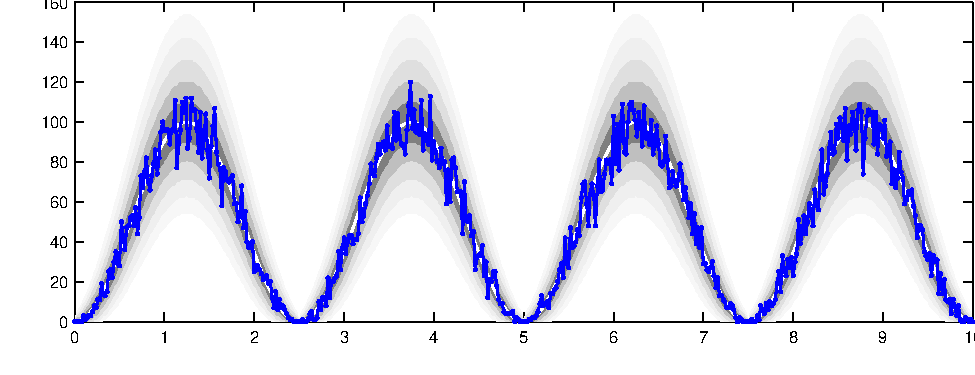
\includegraphics[width=\columnwidth]{figures/cyclostationary-timeseries.pdf}
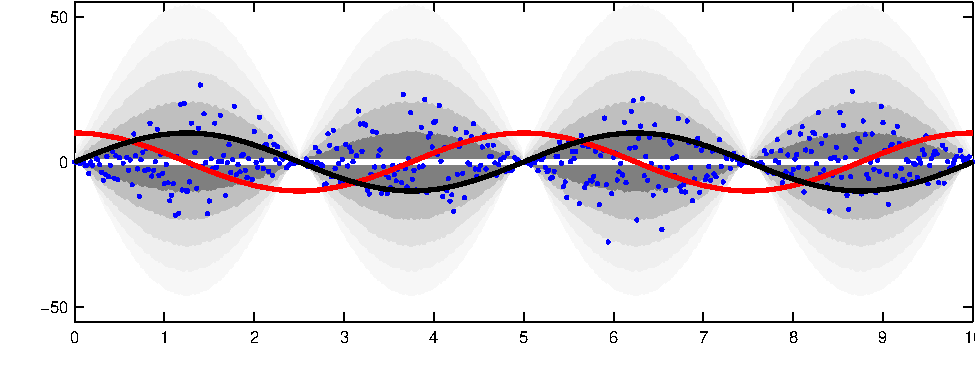
\includegraphics[width=\columnwidth]{figures/cyclostationary-timeseries2.pdf}
\caption{\label{fig:cyclostationary-shot-noise} \textbf{(a)} Model of
  shot noise in the presence of sinusoidal power modulation, as occurs
  in optical heterodyne detection.  The photodiode sees a power
  modulation at $2f_{mod}$ (white) due to the beat between the upper
  and lower modulation sidebands at $f_{carrier} \pm f_{mod}$.
  The gray levels represent the $1\sigma,\ 2\sigma,
  \cdots, 5\sigma$ ranges for a Poisson distribution.  The blue dots
  are a sample realization of this noise. \textbf{(b)} Subtracting the
  mean from (a) leaves only the noise; its bursty nature is obvious.
  Shown in black and red are the I and Q demodulation waveforms,
  respectively.  It is clear that the in-phase demodulation (I)
  samples regions of the time series with higher variance than the
  quadrature phase (Q).  This leads to a higher variance (shot noise
  level) in the I signal and a lower one in the Q signal relative to
  what one would expect from a na\"ive assumption based on the average
  power considered over a whole period of the waveform.}
\end{figure}

\SECTION{Comparison}

In addition to mitigating technical difficulties of RF detection,
homodyne detection confers a fundamental improvement in SNR by up to a
factor of ??. The extra noise in heterodyne detection can be
considered either a result of time dependence in the average power
leading to correlations in the shot
noise\cite{Niebauer1991Nonstationary}, or the simple fact that
demodulation introduces noises from around $2f_{mod}$, giving
an extra dose of shot noise.  A more sophisticated analysis ascribes
this noise to the two heterodyne demodulation quadratures acting as
non-commuting quantum operators\cite{Buonanno2003Quantum}.

\begin{figure}
\centerline{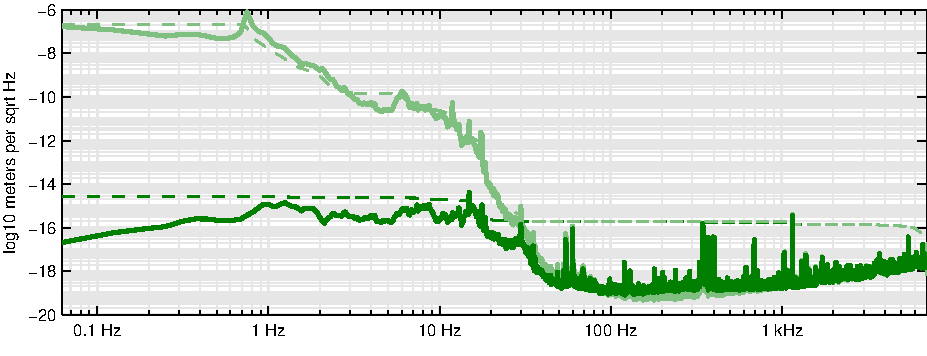
\includegraphics[width=\columnwidth]{figures/residualDARM.pdf}}
\caption{\label{fig:residual-DARM}Residual DARM}
\end{figure}
